\documentclass[11pt]{article}
\usepackage[a4paper,margin=22mm,headheight=16pt]{geometry}
\usepackage{fontspec,xeCJK,xcolor,graphicx,enumitem,fancyhdr,titlesec}
\usepackage{hyperref}
\IfFontExistsTF{Times New Roman}{\setmainfont{Times New Roman}}{\setmainfont{TeX Gyre Termes}}
\IfFontExistsTF{FangSong}{\setCJKmainfont[AutoFakeBold=2]{FangSong}}{\IfFontExistsTF{仿宋}{\setCJKmainfont[AutoFakeBold=2]{仿宋}}{\IfFontExistsTF{FandolFang-Regular.otf}{\setCJKmainfont[AutoFakeBold=2]{FandolFang-Regular.otf}}{\setCJKmainfont{FandolSong-Regular.otf}}}}
\definecolor{ink}{HTML}{173747}\definecolor{accent}{HTML}{227E82}
\hypersetup{colorlinks=true,urlcolor=accent,linkcolor=accent}
\linespread{1.22}\setlength{\parindent}{0pt}\setlength{\parskip}{6pt}
\setlist[itemize]{leftmargin=1.4em,itemsep=3pt}
\titleformat{\section}{\large\bfseries\color{ink}}{}{0pt}{}
\titlespacing*{\section}{0pt}{14pt}{7pt}
\pagestyle{fancy}\fancyhf{}\lhead{\small OMNI LEARNING / 学习手册}\rhead{\small Source-grounded learning}\cfoot{\small\thepage}
\emergencystretch=2em\widowpenalty=10000\clubpenalty=10000
\newcommand{\Needspace}[1]{\par\begingroup\dimen0=#1\relax\vskip0pt plus\dimen0\penalty-100\vskip0pt plus-\dimen0\vskip\dimen0\penalty9999\vskip-\dimen0\vskip0pt\endgroup}
\begin{document}


{\LARGE\bfseries\color{ink} 旅行时看懂夜空：3天学习计划}\par

2026-10-09 | 学习计划 / 3 天\par\vspace{6pt}

\Needspace{5\baselineskip}\section*{你的学习目标与范围}

面向完全零基础、主要在中国旅行的学习者。工具只有肉眼和已有手机星图，不安排器材购买。3天建立一次简单观星所需的判断框架，不以背熟星座或掌握天文学为目标。
完成后，你应能解释恒星与行星的区别，理解月相，并写出一份可执行的肉眼观星准备方案。课程只教通用方法，不预测任何具体日期、地点的可见天象。肉眼加星图即可开始，特殊器材并非入门条件。[S1]

\Needspace{5\baselineskip}\section*{学习路线与时间约定}

Day01 先学会“这个亮点是什么、怎样核对”；Day02 理解月相，并把月光纳入判断；Day03 合并前两天的知识，做一张观星出行卡。下图从左到右对应这三步；中间的四个月面只提示将学习的主要月相，不是当日天象。[S2]
共3天，每天15分钟，包含周末。演示生成开始时间为10:00，时区Asia/Shanghai；这是开始生成的时间，完成检查后再交付。sample\_mode:true，仅记录演示时间，不建立真实定时任务。学习日期由后续实际推进决定，本计划不设置虚构的任务ID。
当前仅提交计划供确认。你批准当前计划后，才会立即开始Day01；确认计划与收到首课是两个步骤。

\begin{center}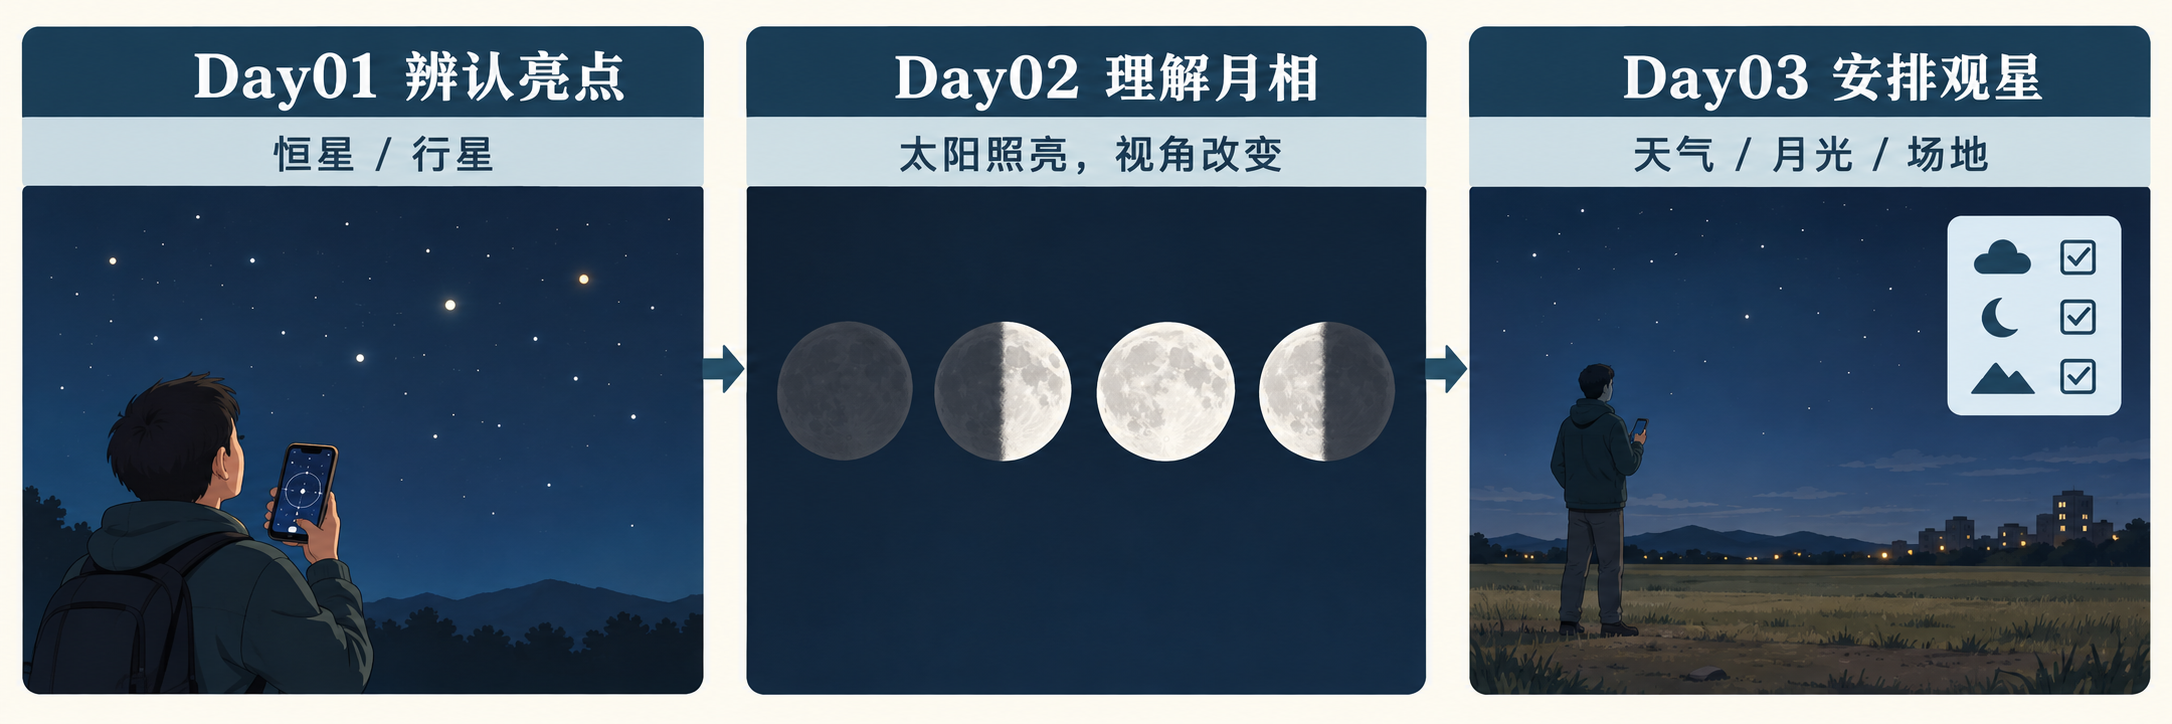
\includegraphics[width=\linewidth,height=0.26\textheight,keepaspectratio]{../assets/figure-7338e8d8739e.png}\par

{\small 图1｜从辨认亮点，到理解月相，再到安排观星。Day02的四个圆盘为主要月相示意，不能用于推算日期或方位。[S2]}\par

{\footnotesize AI生成教学插图（image\_gen，2026-10-09）；非原始证据、非官方图，未使用来源图。完整提示词与检查记录见research/image-record.json。}\end{center}

\Needspace{5\baselineskip}\section*{Day01｜辨认亮点：恒星、行星与手机星图}

当天重点：恒星与行星是什么；肉眼亮点的亮度和闪烁能提供哪些线索；星图如何帮助核对身份。行星往往比恒星更少闪烁，但不能只凭这一个现象下结论。[S6]
时间分配：起点自问1分钟；阅读与看图8分钟；练习4分钟；自检与回顾2分钟，共15分钟。
必做练习：完成2个“线索够不够”的判断情境；在已有星图中找到地点、日期时间和方向显示，记下它们的作用。只检查功能入口，不要求预测本晚或任意指定地点的天象。[S5]
当天产出：一张“先观察、再核对”的小卡，写出恒星与行星的区别，以及为什么“不闪烁”不能直接等同于“行星”。
自检标准：能给出两类天体的区别，并能说出至少两项应核对的星图设置。下一天开头会不看笔记复述这张卡。

\Needspace{5\baselineskip}\section*{Day02｜理解月相：为什么月亮会变形}

先回忆Day01的辨认流程，再学习太阳照明、月球绕地球运动与地面观察视角的关系。月相反映我们看到的受光部分变化；地球影子落在月球上属于月食情形，不能拿来解释普通月相。[S2][S6]
时间分配：闭卷回忆2分钟；阅读与看图7分钟；练习4分钟；核对与回顾2分钟，共15分钟。
必做练习：在教学图中配对新月、上弦月、满月、下弦月；用两句话回答“月亮变形是不是被地球挡住了”。课程不要求3天内实际看到完整月相周期，也不靠“亮面在左或右”作唯一判断。
当天产出：四种主要月相的配对结果与自己的月相解释。
自检标准：四种月相配对正确；解释中同时出现太阳照亮与可见受光比例变化；能把普通月相和月食分开。Day03会再次检索这两点。

\Needspace{5\baselineskip}\section*{Day03｜安排观星：做一张肉眼出行卡}

把辨认流程和月相知识用于出行准备：检查天气、月光、周围灯光和视野，再用星图核对设置。较亮的月光会影响暗弱目标，目标是看月亮还是看更多星星，会改变准备取舍。[S3]
时间分配：回忆前两天2分钟；阅读准备方法6分钟；填写出行卡5分钟；综合自检2分钟，共15分钟。
必做练习：填写一张不绑定日期地点的出行卡，包含天气检查、月光检查、可进入且视野合适的场地、星图设置、一个简单目标、观察记录和阴天备用方案。目标可写“核对一个亮点”或“辨认一种月相”，不预填一定能看到的天体。
当天产出：可在未来旅行前补入当地信息的观星卡。自检标准：七项齐全；能解释两项准备选择的理由；遇到云层或光线不合适时能调整目标。
选做：在实际条件允许时执行出行卡。户外实践另计，不是课程合格前提；充分暗适应可能需要半小时或更久，避免频繁查看亮屏。[S3][S4]

\Needspace{5\baselineskip}\section*{复习、反馈与调整}

Day02开头复习Day01；Day03开头复习Day01与Day02，末尾把概念应用到出行卡。每课练习都将附自检答案和解释，先作答再核对。
最终验收看三项产出：辨认卡、月相解释、观星卡。暂时答不出时，标记具体卡点，下一次先用另一张图或更简单情境重讲，不以“收到PDF”推断已经学会。你可以反馈耗时、难度和手机操作卡点。
15分钟是按阅读、图解和必做练习估算，尚未由你实测。选读链接和夜间观察均另计。计划若需改动，会保留当前版本，另出修订版给你确认。

\Needspace{5\baselineskip}\section*{来源与图片说明}

正文[S1]至[S6]对应文末实际打开的资料。基础概念属于稳定知识；天气、当地可见性和应用界面会随实际情况变化，本计划未核查或断言某次旅行的现场结果。英文资料由课程用中文解释，扩展原文是选读。
路线图为宿主image\_gen模型实际生成的教学插图，不是照片、官方天象图或原始科学证据；星点位置、景观与大小是示意。中间月面从左到右表示新月、上弦月、满月、下弦月的简化形态；显示方向采用本图约定，实际观测方向可能旋转。
联网研究记录、图片生成提示词、来源图授权核查及下载失败记录均保存在本课程research目录。来源图未被下载或嵌入，使用的只有实际生成的路线图。

\Needspace{6\baselineskip}\section*{扩展学习 / Further reading}\small 以下为选读，不计入每日必做时间。\begin{enumerate}[leftmargin=1.6em]

\item [S1] \href{https://science.nasa.gov/skywatching/faq/}{观星常见问题（Skywatching FAQ）} — 读“需要什么工具”和“如何核对可见性”：了解肉眼观星的起点；适合 Day01。\par NASA Science | 发布：未标注 | 核验：2026-10-09

\item [S2] \href{https://science.nasa.gov/moon/moon-phases/}{月相（Moon Phases）} — 读“All Moon Phases”和“Overview From Space”：把月面形状与太阳照明、观察视角联系起来；适合 Day02。\par NASA Science | 发布：未标注 | 核验：2026-10-09

\item [S3] \href{https://science.nasa.gov/solar-system/skywatching/how-to-find-good-places-to-stargaze/}{怎样选择观星地点} — 读月光、场地和到达后的准备三节：用于 Day03 选址与暗适应；不用文中的美国地点作中国观星预测。\par NASA Science / Preston Dyches | 发布：2021-07-28 | 核验：2026-10-09

\item [S4] \href{https://science.nasa.gov/solar-system/skywatching/night-sky-network/may2024-night-sky-notes/}{零器材观星入门} — 读“No Equipment? No Problem!”及手机光线段落：学习星图配合肉眼的方法；跳过特定月份星空图。\par NASA Night Sky Network / Kat Troche（ASP） | 发布：2024-05-01 | 核验：2026-10-09

\item [S5] \href{https://www.jpl.nasa.gov/edu/resources/project/find-planets-in-the-sky/}{用星图寻找行星} — 选读步骤 2、3、5、6：核对星图地点与时间，理解方向和高度；不要求本课程预测某颗行星。\par NASA JPL Education | 发布：未标注 | 核验：2026-10-09

\item [S6] \href{https://science.nasa.gov/skywatching/}{夜空里可以看什么} — 只读“What to Look for in the Sky”的 Planets、Stars：对比行星与恒星的观测线索，跳过当月天象。\par NASA Science | 发布：未标注 | 核验：2026-10-09

\end{enumerate}

\end{document}